\documentclass[hidelinks]{article}

\usepackage[sensei=Nakahara,gakka=Geometry\ in\ Physics,section=Quantum,gakkabbr=QM]{styles/kurisuen}
\usepackage{sidenotes}
\usepackage{van-de-la-sehen-en}
\usepackage{van-de-environnement-en}
\usepackage{boite/van-de-boite-en}
\usepackage{van-de-abbreviation}
\usepackage{van-de-neko}
\usepackage{van-le-trompe-loeil}
\usepackage{cyanide/van-de-cyanide}
\setlength{\parindent}{0pt}
\usepackage{enumitem}
\newlist{citemize}{itemize}{3}
\setlist[citemize,1]{noitemsep,topsep=0pt,label={-},leftmargin=1em}

\usepackage{mathtools}
\usepackage{ragged2e}

\DeclarePairedDelimiter\abs{\lvert}{\rvert}%
\DeclarePairedDelimiter\norm{\lVert}{\rVert}%

% Swap the definition of \abs* and \norm*, so that \abs
% and \norm resizes the size of the brackets, and the 
% starred version does not.
\makeatletter
\let\oldabs\abs
\def\abs{\@ifstar{\oldabs}{\oldabs*}}
%
\let\oldnorm\norm
\def\norm{\@ifstar{\oldnorm}{\oldnorm*}}
\makeatother

\newcommand*{\Value}{\frac{1}{2}x^2}%

\usepackage{fancyhdr}
\usepackage{lastpage}

\fancypagestyle{plain}{%
\fancyhf{} % clear all header and footer fields
\fancyhead[R]{\smash{\raisebox{2.75em}{{\hspace{1cm}\color{lightgray}\textsf{\rightmark\quad Page \thepage/\pageref{LastPage}}}}}} %RO=right odd, RE=right even
\renewcommand{\headrulewidth}{0pt}
\renewcommand{\footrulewidth}{0pt}}
\pagestyle{plain}

\newtheorem*{experiment*}{Measurement}
\newtheorem{example}{Example}
\newtheorem{remark}{Remark}

\def\elementcell#1#2#3#4#5#6#7{%
    \draw node[draw, regular polygon, regular polygon sides=4, minimum height=2cm, draw=cyan, line width=0.4mm, fill=cyan!15!white, #1, inner sep=-2mm](#3) {\Large\textbf{\textsf{\color{cyan!50!black}#4}}};
    \draw (#3.corner 1) node[below left] {\footnotesize{\phantom{Hj}#5}};
    \draw (#3.corner 2) node[below right] {\small{\textsf{#6}}};
    \draw (#3.side 3) node[above] {\footnotesize #7};
    \draw (#3.corner 2) ++ (0,-0.4mm) node(nw#3) {};
    \tcbsetmacrotowidthofnode{\elementcellwidth}{#3}
    \node [fill=cyan, line width=0mm, rectangle, rounded corners=1.8mm, rectangle round south east=false, rectangle round south west=false, anchor=south west, minimum width=\elementcellwidth] at (nw#3) {\small\textsf{\color{white}#2}};
}

\DeclareSIUnit\Dq{Dq}
\usepackage{physics}
\usepackage{bbm}
\newtheorem{lemma}{Lemma}
\newtheorem{proposition}{Proposition}

\DeclareMathOperator{\Pfaffian}{Pf}
\DeclareMathOperator{\sign}{sign}

\begin{document}

\section{Crystal Structure} % (fold)
\label{sec:crystal_structure}

\subsection{Periodic Array of Atoms} % (fold)
\label{sub:periodic_array_of_atoms}

An ideal crystal is constructed by the infinite repetition of identical groups of atoms called the \gloss{basis}. The set of mathematical points to which the basis is attached is called the \gloss{lattice}. The crystal is invariant under a translation
\begin{equation}
    \label{eq:lattice_translation}
    \+vr' = \+vr + u_1 \+va_1 + u_2 \+va_2 + u_3 va_3. 
\end{equation}
The set of points $\+vr'$ defined by the above equation for all integers $u_1$, $u_2$, $u_3$ defines the lattice.
\par
A lattice is said to be \gloss{primitive} if any two points from which the atomic arrangement looks the same can be related by \eqref{eq:lattice_translation}. This also defines the \gloss{primitive translation vectors} $\+va_i$. No cell of smaller volume than $\+va_1 \cdot \+va_2 \times \+va_3$ can serve as the building block for the crystal structure. The \gloss{crystal axes} are defined via primitive translation vectors, which form three adjacent edges of the primitive parallelepiped.
\par
The \gloss{basis} of the crystal structure can be identified once the crystal axes have been chosen.
\par
The parallelpiped defined by primitive axes $\+va_1,\+va_2,\+va_3$ is called a \gloss{primitive cell}. It fills all space by repitition of translation operations. It is also a minimun volume cell. The number of atoms in a primitive cell or a primitive basis is always the same for a given crystal structure.
\begin{figure}[h]
    \centering
    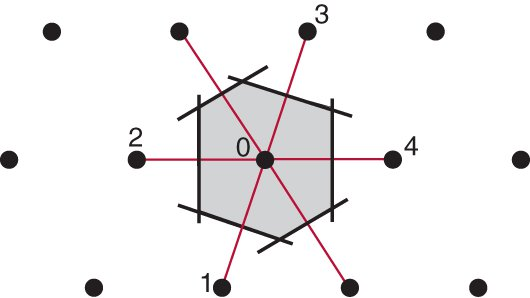
\includegraphics[width=1.5in]{src/WignerSeitz.jpg}
    \caption{Wigner\mbox{-}Seitz Cell.}%
    \label{fig:wigner_seitz}
\end{figure}
\par
The \gloss{Wigner-Seitz} cell is constructed as in \cref{fig:wigner_seitz}.

% subsection periodic_array_of_atoms (end)

\subsection{Fundamental Types of Lattices} % (fold)
\label{sub:fundamental_types_of_lattices}

Lattice \begin{marginwarns}
    No fivefold rotation axis in a lattice.
\end{marginwarns} can be only found such that one-, two-, three-, four- and sixfold rotation axes carry the lattice into itself.
\par
The \gloss[\baselineskip]{point group} is the collection of symmetry operations which carry the lattice into itself.
\begin{sample}
    \begin{example}
        The three $\brac{100}$ axes in a cube are tetrad axes, the four $\brac{111}$ axes are triad axes, and the six $\brac{110}$ axes are diad axes.
    \end{example}
\end{sample}
In the two-dimensional case, a general lattice is known as an \gloss{oblique lattice}, which is invariant under $\pi$ and $2\pi$ about any lattice point. Applying more restrictions may lead to different \gloss{special lattice type}. \gloss[\baselineskip]{Bravais lattice} is the common phrase for a distinct lattice type. There are five bravais lattices in two dimensions.
\par
In \begin{marginwarns}
    In conventional cells there may be more than one lattice sites.
\end{marginwarns} three dimensions there are $14$ different lattice types.
\begin{table}[ht]
    \begin{tabular}{lcl}
        System & Number of lattices & Restrictions on conventional cells and angles \\
        Triclinic & 1 & $a_1 \neq a_2 \neq a_3$,\quad $\alpha\neq \beta\neq \gamma$ \\
        Monoclinic & 2 & $a_1 \neq a_2 \neq a_3$,\quad $\alpha = \gamma = \SI{90}{\degree} \neq \beta$ \\
        Orthorhombic & 4 & $a_1 \neq a_2 \neq a_3$,\quad $\alpha=\beta=\gamma = \SI{90}{\degree}$ \\
        Tetragonal & 2 & $a_1 = a_2 \neq a_3$,\quad $\alpha=\beta=\gamma = \SI{90}{\degree}$ \\
        Cubic & 3 & $a_1 = a_2 = a_3$,\quad $\alpha = \beta = \gamma = \SI{90}{\degree}$ \\
        Trigonal & 1 & $a_1 = a_2 = a_3$,\quad $\alpha = \beta = \gamma < \SI{120}{\degree}, \neq \SI{90}{\degree}$ \\
        Hexagonal & 1 & $a_1 = a_2 \neq a_3$,\quad $\alpha = \beta = \SI{90}{\degree}$,\quad $\gamma=\SI{120}{\degree}$
    \end{tabular}
    \caption{The cubic space lattice.}
\end{table}

% subsection fundamental_types_of_lattices (end)

\subsection{Index System for Crystal Planes} % (fold)
\label{sub:index_system_for_crystal_planes}

\begin{termdef}{Indices of Planes}
    The indices of planes are determined by the following rules:
    \begin{citemize}
        \item Find the intercepts on the axes in terms of the lattice constants $a_1, a_2, a_3$. The axes may be those of a primitive or nonprimitive cell.
        \item Take the reciprocals of these numbers and then reduce to three integers having the same ratio. The result denoted by $\pare{hkl}$ is called the index of the plane.
    \end{citemize}
\end{termdef}
\begin{termdef}{Index of Directions}
    The indices $\brac{uvw}$ are the smallest integers that have the ratio of the components of a vector in the desired direction.
\end{termdef}
\begin{remark}
    In cubic crystals $\brac{hkl}$ is perpendicular to a plane $\pare{hkl}$, but this is not generally true in other crystal systems.
\end{remark}
\begin{finale}
    \begin{proposition}
        One of the lattice planes $\pare{hkl}$ passes through
        \[ \frac{\+va_1}{h},\quad \frac{\+va_2}{k},\quad \text{and}\quad \frac{\+va_3}{l}, \]
        provided that $\gcd\pare{h,k,l} = 1$.
    \end{proposition}
\end{finale}
\begin{proof}
    We demand integer solutions $\pare{r,s,t}$ to
    \[ rh + sk + tl = 1, \]
    the existence of which is guaranteed by B\'ezout's theorem.
\end{proof}

% subsection index_system_for_crystal_planes (end)

\subsection{Simple Crystal Structures} % (fold)
\label{sub:simple_crystal_structures}

\subsubsection{Sodium Chloride Structure} % (fold)
\label{ssub:sodium_chloride_structure}

\ce{NaCl} is of fcc lattice, whose basis consists of one \ce{Na+} ion and one \ce{Cl-} ion separated by one-half the body diagonal of a unit cube.

\begin{figure}[ht]
    \centering
    \includegraphics[width=8cm]{src/NaCl.png}
    \caption{NaCl Structure.}
\end{figure}

% subsubsection sodium_chloride_structure (end)

\subsubsection{Cesium Chloride Structure} % (fold)
\label{ssub:cesium_chloride_structure}

\ce{CsCl} is of sc lattice, whose basis consists of one \ce{Cs+} ion and one \ce{Cl-} ion, the latter of which lies in the bcc position.

\begin{figure}[ht]
    \centering
    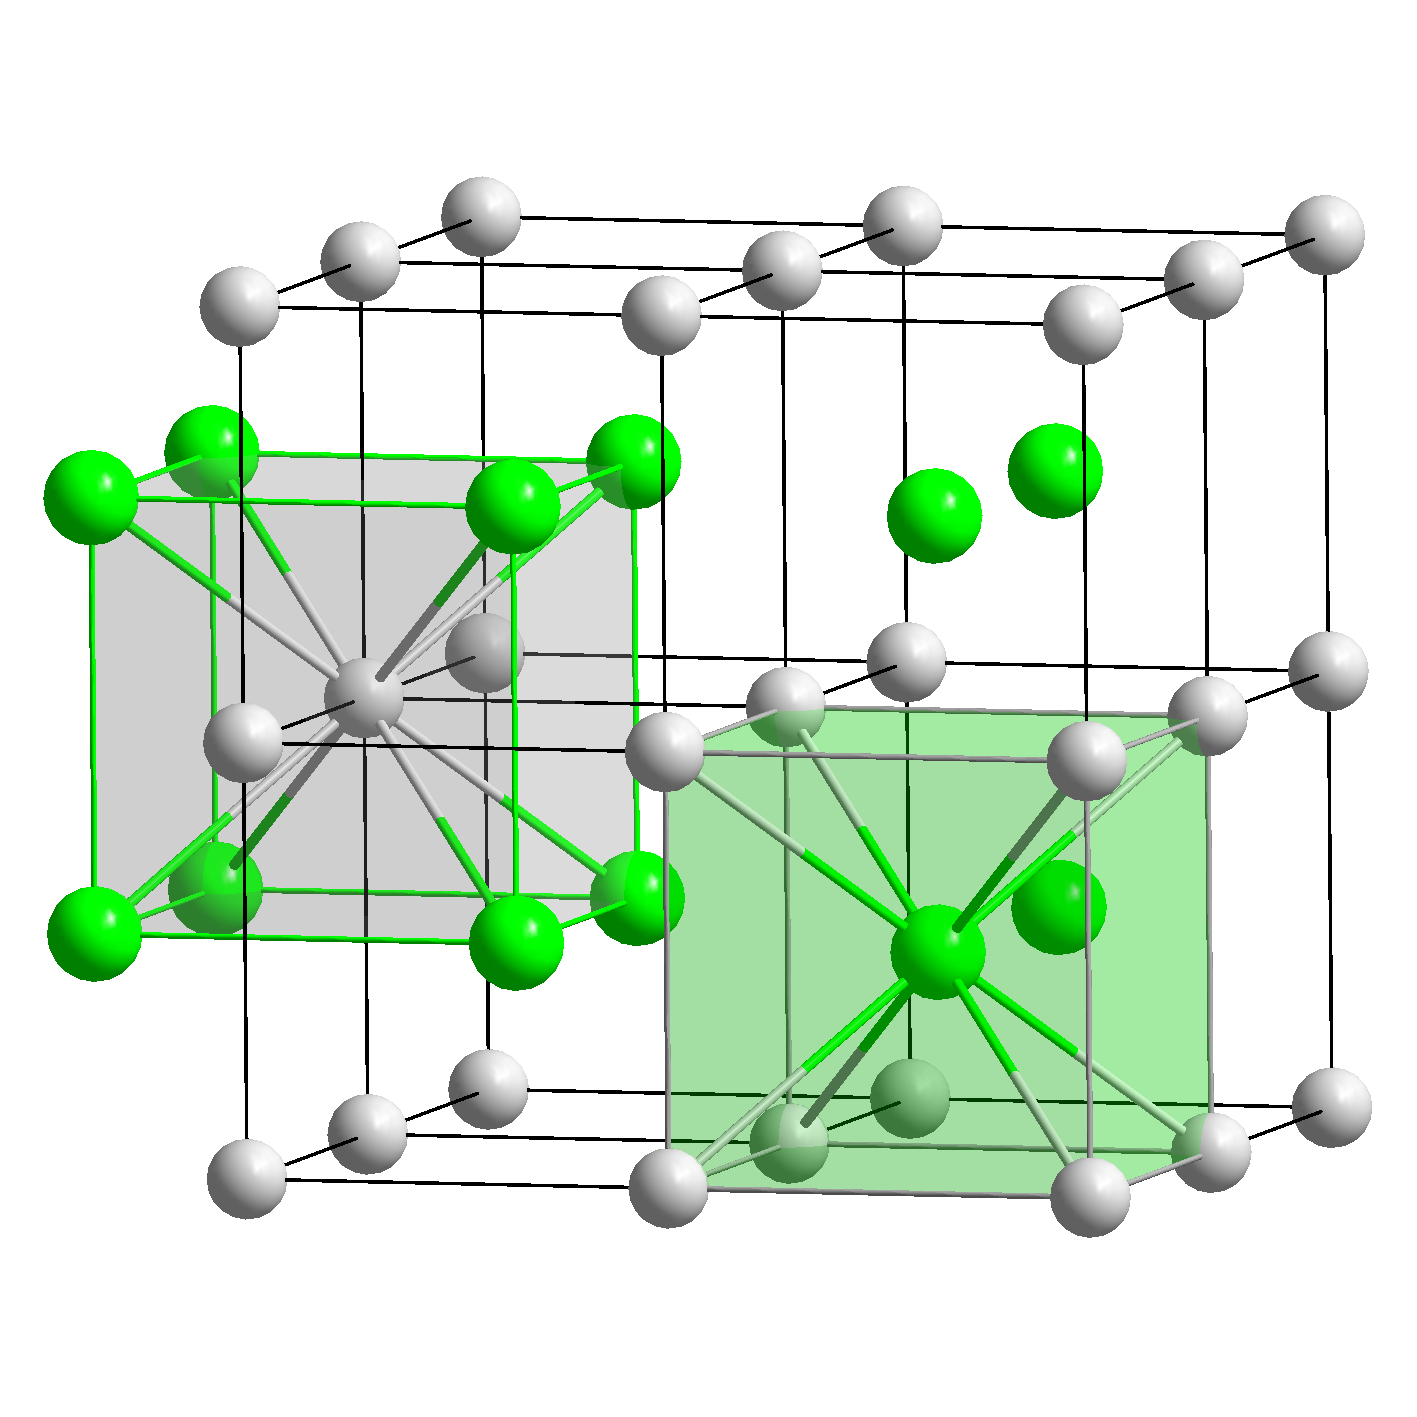
\includegraphics[width=6cm]{src/CsCl.png}
    \caption{CsCl Structure.}
\end{figure}

% subsubsection cesium_chloride_structure (end)

\subsubsection{Hexagonal Close-Packed Structure} % (fold)
\label{ssub:hexagonal_close_packed_structure}

Layer $A$ is arranged by placing each sphere in contact with six others in a plane. This may be the basal plane of the hcp structure or the $\pare{111}$ plane of the fcc sturcture.
\par
The second laybe $B$ is added by placing each sphere of $B$ in contact with three spheres of the bottom layer. Then the layer $C$ is added by either of the following ways:
\begin{citemize}
    \item added over the holes in the first layer that are not occupied by $B$, whence we obtain the fcc structure; or
    \item placed directly over the centers of the spheres in the first layer.
\end{citemize}

% subsubsection hexagonal_close_packed_structure (end)

\subsubsection{Diamond Structure} % (fold)
\label{ssub:diamond_structure}

The space lattice of diamond is face-centered cubic. The primitive basis of the diamond structure has two identical atoms at coordinates $\pare{0,0,0}$ and $\displaystyle \pare{\rec{4},\rec{4},\rec{4}}$.

% subsubsection diamond_structure (end)

\subsubsection{Cubic Zinc Sulfide Structure} % (fold)
\label{ssub:cubic_zinc_sulfide_structure}

In the \ce{ZnS} structure, the \ce{Zn} atoms are placed on the fcc lattice, and \ce{S} atom on the other fcc lattice.

% subsubsection cubic_zinc_sulfide_structure (end)

% subsection simple_crystal_structures (end)

\subsection{Nonideal Crystal Structures} % (fold)
\label{sub:nonideal_crystal_structures}

\gloss{Random stacking} occurs if the stacking sequence of close-packed planes is random.
\par
\gloss{Polytypism} is characterized by a stacking sequence with a long repeat unit along the stacking axis.

% subsection nonideal_crystal_structures (end)

% section crystal_structure (end)

\end{document}
